% !TEX encoding = UTF-8
\documentclass[a4paper,oneside,openright,titlepage,10pt,footinclude,headinclude]{scrbook}
\usepackage[T1]{fontenc}
\usepackage[parts]{classicthesis}
\usepackage{hyperref}
\usepackage[utf8]{inputenc}
\usepackage[swapnames]{frontespizio}
\usepackage[italian]{babel}
\usepackage{amsfonts,amsmath,amssymb,graphicx,amsthm}
\usepackage{listings}
\usepackage[framemethod=TikZ]{mdframed}
\usepackage{color}

\definecolor{light-gray}{gray}{0.95}

%% Generic use box with grey background
\newmdenv[%
	backgroundcolor=light-gray,
	roundcorner=5pt,
	leftmargin=1,
	rightmargin=1,
	innerleftmargin=15, 
	innertopmargin=5,
	innerbottommargin=5,
	outerlinewidth=1,
	linecolor=light-gray,
]{graybox}

\lstset
{	language=Python,
	basicstyle=\small\ttfamily,
	keywordstyle=\color{red},
	commentstyle=\color{blue}, 
	tabsize=2, 
	frame=none,
	showstringspaces=false,
	basicstyle=\fontsize{9}{9}\selectfont,
	columns=fullflexible,
	captionpos=b,
}
\begin{document}

\begin{frontespizio}
\Universita{Verona}
\Facolta{Scienze Matematiche, Fisiche e Naturali}
\Corso[Laurea Magistrale]{Ingegneria e Scienze Informatiche}
\Titoletto {Progetto corso Sicurezza del Software}
\Titolo {Offuscatore per il linguaggio Python}
\Candidato[VR419955]{Giovanni Bellorio}
\Candidato[VR424301]{Kevin Costa}
\Candidato[VR420117]{Alessandro Cosma}
\Annoaccademico{2018-2019}
\end{frontespizio}

\tableofcontents

%% INTRODUZIONE
\chapter{Introduzione}\label{introduzione}

Lo scopo di questo progetto è realizzare un offuscatore per il linguaggio Python. Il programma che implementa l'offuscatore sarà realizzato anch'esso in Python e prenderà in considerazione le seguenti tipologie di offuscamento del codice:
\begin{itemize}
\item
\textbf{Layout obfuscation}
\item
\textbf{Data obfuscation}
\item
\textbf{Control Flow obfuscation}
\end{itemize}
Nel capitolo \ref{background} daremo una panoramica generale sui concetti legati all'offuscamento del codice, spiegando cos'è formalmente un offuscatore, quali sono le sue carateristiche, i suoi pregi e i suoi difetti, infine spiegheremo nel dettaglio le varie tecniche di offuscamento che andremo ad utilizzare.

Nel capitolo \ref{offuscatore} verrà presentato il nostro programma per l'offuscamento del codice. Elencheremo le varie scelte progettuali effettuate in fase di progettazione (\ref{offuscatore_scelte}) e successivamente presenteremo passo passo il codice che implementa l'algoritmo (\ref{offuscatore_algo}). 

Infine, nel capitolo \ref{esempio}	mostreremo un semplice esempio del suo fuzionamento accompagnato da alcuni test.

%% BACKGROUND
\chapter{Background}\label{background}

Quando si considera un software sviluppato e distribuito, la maggior parte del suo ``know-how'' risiede nel prodotto stesso. Risulta quindi essenziale la protezione del suo codice e della sua proprietà intellettuale. \medskip


Attacchi di \emph{reverse-engineering} hanno l'obiettivo di attuare analisi statiche e dinamiche del codice, al fine di capire il funzionamento interno di un programma proprietario di interesse. La protezione è necessaria ad ogni livello di funzionamento del programma, a partire dal codice sorgente, fino ad arrivare al codice macchina, passando anche per le informazioni di interesse che il programma da proteggere scambia con l'ambiente di esecuzione.\medskip

\noindent Esistono varie tecniche di protezione del codice con differenti obiettivi:
\begin{itemize}
\item
\emph{Misure legali}: leggi, copiright, patenti, brevetti e licenze ideate per proteggere la ``forma'' e l'idea di un programma.
\item
\emph{Offuscamento}: rendere difficile il reverse-engineering del programma.
\item
\emph{Watermarking del software}: inserire una firma o un riconoscimento contro il furto del programma.
\item
\emph{Tamper-proofing}: rilevare violazioni contro l'integrità del codice o modifiche illegali.
\end{itemize}

Essendo il nostro progetto mirato alla realizzazione di un offuscatore per codice Python, descriveremo ora in dettaglio il concetto di offuscatore e presenteremo alcune delle principali tecniche utilizzate. 

\section{Offuscatore}

Sia:  
\begin{center}
$P \xrightarrow{T} P^{'}$
\end{center}
una trasformazione di un programma sorgente $P$ in un programma $P^{'}$
con $P, P^{'} \in Programs$, cioè l'insieme dei programmi.\medskip


\noindent $P \xrightarrow{T} P^{'}$ è una trasformazione di offuscamento se $P$ e  $P^{'}$ hanno lo stesso \emph{comportamento osservabile}.

Più precisamente, affinchè $P \xrightarrow{T} P^{'}$ sia una trasformazione di offuscamento legale, devono valere le seguenti condizioni:
\begin{enumerate}
\item
Se $P$ non riesce a terminare o termina in una condizione di errore, allora $P^{'}$ può o non può terminare.
\item
Altrimenti, $P^{'}$ deve terminare e produrre lo stesso output di $P$.
\end{enumerate}

Il \emph{livello di sicurezza} rispetto al reverse-engineering che un offuscatore aggiunge  ad un dato programma dipende da vari fattori: raffinatezza della trasformazione di offuscamento, potenza del deoffuscatore, quantità di risorse  (tempo e memoria) disponibili al deoffuscatore.\\

\subsection{Impossibilità di offuscare un programma}

Una trasformazione di offuscamento non potrà mai proteggere completamente un programma.
Fred Cohen, il primo ad introdurre la diversità dei programmi come difesa contro gli attacchi automatici ai sistemi operativi, affermava che: \smallskip

\textit{“Any protection scheme other than a physical one depends on the operation of a finite state machine, and ultimately, any finite state machine can be examined and modified at will, given enough time and effort. The best we can ever do is delay the attack by increasing the complexity of making desired alterations (security through obscurity)”}\smallskip

[inserire risultati paper ``On the impossibility of code obfuscation'']


\subsection{Valutare le trasformazioni offuscanti}
Una trasformazione offuscante è valutate in base alle seguenti proprietà:
\begin{itemize}
\item
\textbf{Potenza}: quanto più difficile è comprendere il codice offuscato rispetto a quello originale.
\item
\textbf{Resilienza}: misura quanto una trasformazione regge l'attacco di un deoffuscatore automatico.
\item
\textbf{Costo}: misura quanto overhead computazionale (tempo e spazio) viene aggiunge all'applicazione offuscata.
\item
\textbf{Furtività}: misura quanto bene il codice nuovo introdotto con la trasformazione si integra con il codice originale.
\end{itemize}

\paragraph{Potenza} 
Sia $T$ una trasformazione che preserva il comportamento, tale che $P \xrightarrow{T} P^{'}$ trasfroma un programma $P$ in un programma $P^{'}$. Sia $E(P)$ la complessità di $P$.\smallskip


$T_{pot}(P)$, la potenza di $T$ rispetto ad un programma $P$, è una  misura del grado con cui $T$ cambia la complessità di $P$.

\begin{center}
$T_{pot}(P) = E(P^{'}) / E(P) - 1$
\end{center}
 
 $T$ è una \emph{trasformazione di offuscamento potente} se $T_{pot}(P) > 0$.
 
 \paragraph{Resilienza} 
Sia $T$ una trasformazione che preserva il comportamento, tale che $P \xrightarrow{T} P^{'}$ trasfroma un programma $P$ in un programma $P^{'}$.  $T_{res}(P)$ è la \emph{resilienza} di $T$ rispetto ad un programma $P$. \smallskip

 $T_{res}(P) = one-way$ se l'informazione è rimossa da $P$ tale che $P$ non può essere ricostruito da $P^{'}$. \smallskip

\begin{center}
$T_{res} = Resilience(T_{Deobfuscator\_effort}, T_{Programmer\_effort})$ 
\end{center}


\paragraph{Costo}
Il costo di una trasformazione offuscante è il tempo di esecuzione (o la quantità di spazio occupato) del programma offuscato rispetto a quello originale.\smallskip

\noindent $T_{cost}(P)$, cioè il costo di un programma P, può essere classificato su una scala di quattro punti come segue:
\begin{itemize}
\item
\textbf{caro}: se l'esecuzione di $P^{'}$ richiede esponenzialmente più risorse di $P$.
 \item
\textbf{costoso}: se l'esecuzione di $P^{'}$ richiede $O(n^{p}), p>1$ risorse più di $P$.
 \item
\textbf{economico}: se l'esecuzione di $P^{'}$ richiede $O(n)$ risorse più di $P$.
 \item
\textbf{gratuito}: se l'esecuzione di $P^{'}$ richiede $O(1)$ risorse più di $P$.
\end{itemize}


 \paragraph{Furtivita}
 Mentre una trasformazione resiliente potrebbe non essere suscettibile agli attacchi di deoffuscatori automatici, potrebbe comunque essere suscettibile agli attacchi degli umani.
 
In particolare, se una trasformazione introduce un nuovo codice che differisce ampiamente da ciò che è presente nel programma originale, sarà facile individuare per un reverse engineer. Tali trasformazioni non sono furtive (a.k.a. \emph{unstealthy}).

La furtività è una nozione sensibile al contesto. Il codice può essere nascosto in un programma ma estremamente visibile in un altro.\\

\section{Tecniche di offuscamento del codice}
In questa sezione andremo a descrivere a livello teorico le tecniche di offuscamento che saranno utilizzate successivamente all'interno del nostro offuscatore.

\subsection{Layout Obfuscation}
L'obiettivo del \emph{Layout Obfuscation} è cambiare o rimuove le informazioni utili dal codice senza influire sulle istruzioni reali.\medskip


\noindent Tecniche principali utilizzate per questo tipo di offuscamento:
\begin{itemize}
\item
\textbf{Rimozione commenti}: vengono rimossi i commenti e i docstring presenti nel codice.
\item
\textbf{Rinominazione degli identificatori }: i nuovi nomi possono utilizzare diversi schemi, numeri, caratteri non stampabili o caratteri invisibili. Inoltre i nomi possono essere riutilizzati, purchè usati in ambiti diversi.
\end{itemize}

\noindent Queste sono trasformazioni \emph{one-way} in quanto la formattazione originale non può essere ripristinata.\medskip

Vantaggi: 
\begin{itemize}
\item[-]
potente contro l'attacco umano
\item[-]
per quanto riguarda i costi è gratuito.
\item[-]
è molto utile per offuscare \emph{authorship} del codice.
\end{itemize}

Svantaggi:
\begin{itemize}
\item[-]
Ha una bassa potenza, in quanto nella formattazione c'è poco contenuto semantico. 
\end{itemize}


\subsection{Control Flow Obfuscation}
Il \emph{Control Flow Obfuscation} trasforma un control-flow ben strutturato di un programma eseguibile in una struttura difficile da analizzare da un programma che rileva le trasformazioni del control-flow. Tale offuscamento può ostruire e fermare gli attacchi statici al control-flow del codice eseguibile sotto attacchi di tipo white-box. Questa tecnica costringe l'attaccante ad eseguire attacchi dinamici per ottenere il control-flow, in questo modo diventa molto più difficile da ottenere e aumenta significativamente lo sforzo dell'attacco.

\noindent Tecniche principali utilizzate per questo tipo di offuscamento:
\begin{itemize}
\item
\textbf{Predicati opachi}: sono espressioni di valore booleano per le quali il difensore sa se restituiranno true, false o talvolta true e talvolta false
\item
\textbf{CFG Riducibili}: sono grafi che possono essere ridotti a un singolo nodo mediante una sequenza di applicazioni di due regole
\item
\textbf{Predicati opachi dinamici}: una famiglia di predicati opachi correlati, che valutano tutti lo stesso risultato ad ogni esecuzione, ma in diverse esecuzioni possono valutare risultati diversi
\end{itemize}

Vantaggi: 
\begin{itemize}
\item[-]
potente contro l'analisi statica
\item[-]
difficili da valutare dall'attaccante per la complessità esponenziale
\item[-]
è molto utile per offuscare \emph{authorship} del codice.
\end{itemize}

Svantaggi:
\begin{itemize}
\item[-]
Vulnerabile all'analisi dinamica 
\end{itemize}

\subsection{Data Obfuscation}
Per offuscare una variabile \textit{v} in un programma, la si converte dalla rappresentazione scelta inizialmente dal programmatore ad un rappresentazine più difficile da analizzare per l'attaccante. Qualsiasi valore che una variabile \textit{v} può assumere deve essere
rappresentato nella nuova variabile offuscata. Si ha bisogno di due funzioni: 

\begin{center}
encode $ \medskip E: T \xrightarrow{} T'$
\end{center}

\begin{center}
decode $ D: T' \xrightarrow{} T$
\end{center}

e le operazioni sulle variabili devono essere interpretate nella nuova rappresentazione.

\noindent Tecniche principali utilizzate per questo tipo di offuscamento:
\begin{itemize}
\item
\textbf{Encoding Integers}: gli interi possono essere codificati con "trucchi" della teoria dei numeri o criptandoli.
\item
\textbf{Encoding Booleans}: si usa lo stesso approccio per l'\textit{Encoding Integers}, ma è molto più semplice perchè il range dei loro valori è conosciuto
\item
\textbf{Encoding Literal Data}: possibili soluzioni possono essere scomporre i dati in parti più piccole e nasconderle nel programma, fare lo \textit{xor} di una stringa con un valore costante conosciuto o usare macchine di Mealy.
\item
\textbf{Encoding Arrays}: si possono riordinare o ristrutturare gli elementi dell'array
\end{itemize}


Vantaggi: 
\begin{itemize}
\item[-] potente contro l'attacco umano.
\item[-] per quanto riguarda i costi è gratuito.
\item[-] i \textit{Literal Data} contengono molte informazioni semantiche.
\end{itemize}

Svantaggi:
\begin{itemize}
\item[-] rallentamento delle prestazioni per le continue decodifiche.
\end{itemize}
 

%% OFFUSCATORE
\chapter{Offuscatore per Python}\label{offuscatore}

\section{Scelte progettuali}\label{offuscatore_scelte}


\subsection{Assunzioni}
Per l'offuscatore che abbiamo crato sono state fatte le seguenti assunzioni:
\begin{itemize}
\item[-] Essendo python un linguaggio di programmazine non tipato, quando faccio l'encoding in una macchina di Mealy subito dopo faccio il decoding perché se in una condizione \textit{if} entro nel ramo \textit{else} e viene cambiato tipo di una variabile (da stringa a intero), non riesco più a trattarla come stringa, ma dorò trattarla come array permutation.
\item[-] Nell'array permutation assumiamo che l'array contenga dei valori e non dei nomi di variabili, altrimenti bisognerebbe andare in profondità.
\item[-] Nel Control Flow Obfuscation assumiamo di inserire i predicati opachi non prima di una riga che termini con ":", per evitare possibili errori di indentazione nell'inserimento del predicato opaco.
\end{itemize}   

\section{Algoritmo e codice}\label{offuscatore_algo}
Viene ora presentato il codice che implementa l'offuscatore.\medskip

Il codice sorgente è composto da  un metodo \texttt{main()} che rappresenta l'entry point del nostro programma e da una serie di funzioni  che vengono invocate all'interno di tale metodo per svolgere le funzioni di offuscamento.
\begin{graybox}[innerleftmargin=2,]
\begin{lstlisting}
def main():

    print("-----------------------------------")
    print("OBFUSCATION STARTED\n")

    name_src = sys.argv[1]  # name of the source file, passed as argument
    name_dest = name_src+"_OBFUSCATED.py"  # name of the destination file

    file_SRC = open(name_src, "r")
    file_DEST = open(name_dest, "w")

    # Call 'remove_comments_and_docstrings()' function on the source file object
    # which it is first converted to a string through the read() method.
    # 'out' contains a string with the entire code
    out = remove_comments_and_docstrings(file_SRC.read())   

    # Call 'opaque_predicate()' function
    out = opaque_predicate(out)

    # Call 'encoding_literal_data()' function
    out = encoding_literal_data(out)

    # Call 'obfuscate_variables()' function
    out = obfuscate_variables(out)
    
    # Call 'obfuscate_functions()' function
    out = obfuscate_functions(out)

    # Write the result into file_DEST
    file_DEST.write(out)
    file_DEST.close()
    file_SRC.close()

    print("\nOBFUSCATION ENDED")
    print("-----------------------------------")


if __name__ == '__main__':
    main()
\end{lstlisting}
\end{graybox}

All'inizio dell'esecuzione del programma, viene letto il nome del file sorgente, contenente il software Python da offuscare e salvato nella variabile \texttt{name\_src}: questa informazione deve essere passata come argomento di input all'offuscatore, con una sintassi del tipo:
\begin{graybox}
\begin{lstlisting}[language=bash,basicstyle=\fontsize{10}{9}\selectfont,]
python3  		offuscatore.py 	<nome_file_da_offuscare>.py
\end{lstlisting}
\end{graybox}
\noindent dove \texttt{offuscatore.py} è il nome dell' offuscatore e \texttt{<nome\_file\_da\_offuscare>} è il nome del file di input.

Successivamente viene aperto in sola lettura il file sorgente (variabile \texttt{file\_SRC}) e viene creato un nuovo file, chiamato come il precedente ma con l'aggiunta della suffisso ``OBFUSCATED''  e salvato nella variabile \texttt{file\_DEST}: esso rappresenta il file che conterrà l'output del nostro programma cioè il software offuscato.\smallskip

\noindent In seguito vengono chiamate in sequenza le seguenti funzioni:
\begin{itemize}
\item
\textbf{remove\_comments\_and\_docstrings()}: esegue un \emph{layout obfuscation} rimuovendo i commenti e la documentazione;
\item
\textbf{opaque\_predicate()}: esegue un \emph{control flow obfuscation}, inserendo predicati opachi; 
\item
\textbf{encoding\_literal\_data()}: esegue un \emph{data obfuscation}, codificando stringhe, array e interi;
\item
\textbf{obfuscate\_variables()}: esegue un \emph{layout obfuscation}, rinominando i nomi di variabili;
  \item
\textbf{obfuscate\_functions()}: esegue un \emph{layout obfuscation}, rinominando i nomi di funzione e il relativo ``corpo''.
\end{itemize}
Ognuna di queste funzioni riceve in input il programma (variabile \texttt{out}) trasformato dalla funzione di offuscamento precedente, vi applica un certo insieme di trasformazioni offuscanti e successivamente restituisce un output trasformato, che viene poi dato in input alla funzione di offuscamento successiva.\smallskip

Alla fine del metodo \texttt{main()}, viene scritto nel file di output il programma offuscato  e vengono chiusi i file di input e output precedentemente aperti.


\subsection{Codice di Layout Obfuscation}

\subsubsection{remove\_comments\_and\_docstrings()}

La prima funzione di layout obfuscation è \emph{remove\_comments\_and\_docstrings}.
Questa funzione ha l'obiettivo di eliminare dal codice sorgente tutti i commenti  e tutte le stringhe relative alla documentazione del codice presenti al suo interno.
\begin{graybox}[innerleftmargin=2,]
\begin{lstlisting}
def remove_comments_and_docstrings(source):
    """
    Returns 'source' minus comments and docstrings.
    """

    print("-> removing comments and docstrings")

    io_obj = StringIO(source)
    out = ""
    prev_toktype = tokenize.INDENT
    last_lineno = -1
    last_col = 0
    myline = ""
    is_junk = False

    for tok in tokenize.generate_tokens(io_obj.readline):
        token_type = tok[0]
        token_string = tok[1]
        start_line, start_col = tok[2]
        end_line, end_col = tok[3]
        ltext = tok[4]
        # The following two conditionals preserve indentation.
        # This is necessary because we're not using tokenize.untokenize()
        # (because it spits out code with copious amounts of oddly-placed
        # whitespace).
        if start_line > last_lineno:
            last_col = 0
        if start_col > last_col:
            myline += (" " * (start_col - last_col))
        # Remove comments:
        if token_type == tokenize.COMMENT:
            is_junk = True
            pass
        # This series of conditionals removes docstrings:
        elif token_type == tokenize.STRING:
            if prev_toktype != tokenize.INDENT:
        # This is likely a docstring; double-check we're not inside an operator:
                if prev_toktype != tokenize.NEWLINE:
                    # Note regarding NEWLINE vs NL: The tokenize module
                    # differentiates between newlines that start a new statement
                    # and newlines inside of operators such as parens, brackes,
                    # and curly braces.  Newlines inside of operators are
                    # NEWLINE and newlines that start new code are NL.
                    # Catch whole-module docstrings:
                    if start_col > 0:
                        # Unlabelled indentation means we're inside an operator
                        myline += token_string
                    # Note regarding the INDENT token: The tokenize module 
                    # does not label indentation inside of an operator (parens,
                    # brackets, and curly braces) as actual indentation.
                    # For example:
                    # def foo():
                    #     "The spaces before this docstring are tokenize.INDENT"
                    #     test = [
                    #         "The spaces before this string do not get a token"
                    #     ]
                    else:
                        is_junk = True
                else:
                    is_junk = True
            else:
                is_junk = True
        else:
            myline += token_string

        if token_type == tokenize.NEWLINE or token_type == tokenize.NL:
            if not (is_junk and re.match(r'^\s*$', myline)):
                out += myline
            myline = ""
            is_junk = False

        prev_toktype = token_type
        last_col = end_col
        last_lineno = end_line
    return out
\end{lstlisting}
\end{graybox}
Questa funzione sfrutta il modulo \texttt{tokenize} il quale  fornisce uno scanner lessicale per codice sorgente Python.
Essa preserva l'indentazione del codice, essenziale per il corretto funzionamento di un programma Python, inoltre, ogni qual volta una  riga viene ``svuotata'' di tutti suoi token perchè non vi è presenta nessuna istruzione, quest'ultima viene eliminata dal codice per non lasciare inutili spazi vuoti.

\subsubsection{obfuscate\_variables()}\label{obfuscate_variables}

La seconda funzione che esegue il layout obfuscation è \emph{obfuscate\_variables}.
La funzione prende in input il codice del programma da offuscare (variabile \texttt{out}) e ritorna il medesimo codice con i nomi delle variabili offuscate.\medskip


\noindent Riportiamo il codice:
\begin{graybox}[innerleftmargin=2,]
\begin{lstlisting}
def obfuscate_variables(out):
    """
        Returns 'source' code with variables offuscated.
    """

    print("-> obfuscating variables")

    # Tree object contains the AST of the code
    tree = ast.parse(out)

    # Extraction of all variables defined
    variables = get_variables(tree)

    # Choose new names
    for variable in variables:
        VARIABLES_DICT[variable] = random_sequence()

    # Renomination of all variable occurrences
    tree = rename_variables(tree, VARIABLES_DICT)

    # Convert the new AST to a valid code
    return astor.to_source(tree)
\end{lstlisting}
\end{graybox}

Attraverso il comando \texttt{ast.parse(out)}, il codice contenuto nella variabile \texttt{out} viene convertito in una struttura ad albero e salvata nella variabile \texttt{tree}. Questo albero rappresenta l'\emph{abstract syntax tree} del codice sorgente del programma dato in input.

Successivamente vengono estratte tutte le variabili presenti nel programma, attraverso la funzione \texttt{get\_variables()} e salvate nella lista \texttt{variables}. Ad ognuna di esse viene poi associato un nuovo nome casuale, utilizzando la funzione \texttt{random\_sequence()}.\\
L'associazione tra il nome della variabile originale e il nuovo nome viene salvata nel dizionario \texttt{VARIABLES\_DICT}, definito come variabile globale.

Infine, tramite la funzione \texttt{rename\_variables()}, viene applicata la ridenominazione delle variabili sulla base delle associazioni precedentemente stabilite.

Viene quindi ritornato il codice sorgente del programma, invocando la funzione  \texttt{astor.to\_source(tree)}, che prende come input l'abstract syntax tree, su cui sono state apportate le precedenti trasformazioni offuscanti e ritorna come output il relativo codice sorgente. Questo metodo, che trasforma un abstract syntax tree nel corrispettivo codice sorgente, appartiene al modulo \texttt{astor}, esterno alla libreria Python.\bigskip


Riportiamo ora il codice delle funzioni \texttt{get\_variables()}, \texttt{random\_sequence()} e \texttt{rename\_variables()}, seguito da una breve descrizione.\smallskip

La funzione \texttt{get\_variables()} prende come input un abstract syntax tree e ritorna come output un dizionario, contenente ogni variabile presente nell albero (\emph{key}) e il relativo tipo (\emph{value}).
\begin{graybox}[innerleftmargin=2,]
\begin{lstlisting}
def get_variables(tree):
    """
    :param tree:
    :return: a dictionary contains each variable (key) and its type (value) 
    contained in the code (passed as AST 'tree')
    """

    variables = {}

    for node in ast.walk(tree):
        # Saved variables declared
        if isinstance(node, ast.Assign) and isinstance(node.targets[0], ast.Name):
            if node.targets[0].id not in variables:
                    variables[node.targets[0].id] = type(node.value).__name__
        if isinstance(node, ast.Attribute):
            if isinstance(node.value, ast.Name):
                if node.value.id == "self":
                    variables[node.attr] = type(node.attr).__name__
        
    return variables
\end{lstlisting}
\end{graybox}

La funzione esegue una visita dell'albero, svolta tramite il metodo \texttt{ast.walk()}. In questo caso vengono presi in considerazione i nodi dell'albero che rappresentano un assegnamento (\texttt{ast.Assign}) oppure un attributo (\texttt{ast.Attribute}); quest'ultimo caso è necessario in presenza di una definizione di classe, in cui una variabile viene anteceduta dal prefisso \texttt{self}.

I nomi di variabili e il loro tipo vengono salvati nel dizionario \texttt{variables}, ritornato come output dalla funzione.\bigskip

La funzione \texttt{random\_sequence()} genera una sequenza casuale di 23 caratteri, scelti in un alfabeto di soli due elementi: il numero `\texttt{0}' oppure la lettera `O'. La sequenza creata è sempre diversa dalla precedenti sequenze generate.
\begin{graybox}[innerleftmargin=2,]
\begin{lstlisting}
def random_sequence():

    seq = generate_sequence()

    if seq not in RANDOM_SEQUENCES_SET:
        RANDOM_SEQUENCES_SET.add(seq)
        return seq
    else:
        random_sequence()

def generate_sequence():

    cryptorand = SystemRandom()

    sequence = []

    for i in range(22):
        flip = random.randint(1, 2)
        if flip == 1:
            sequence.append("0")
        else:
            sequence.append("O")

    random.seed()
    cryptorand.shuffle(sequence)

    return "O"+"".join(sequence)
\end{lstlisting}
\end{graybox}

Questa funzione utilizza il metodo \texttt{generate\_sequence()} per generare la sequenza. Quest'ultimo utilizza il modulo \texttt{randint} e \texttt{SystemRandom} della libreria \texttt{random}.  Ogni sequenza generata, prima di essere ritornata alla funzione \texttt{random\_sequence()}, viene mescolata tramite il metodo \texttt{cryptorand.shuffle()}: questo ci permette di avere meno probabilità di generare dupliacati.

Successivamente, se la sequenza generata è una sequenza valida (non è un duplicato), viene salvata nell'insieme \texttt{RANDOM\_SEQUENCES\_SET}, definito come globale e ritornata come output dalla funzione; altrimenti viene scartata e ne viene generata una nuova.\bigskip

La funzione \texttt{rename\_variables()} prende in input un abstract sintax tree (parametro \texttt{tree}) e un dizionario contenente le associazioni tra nomi originali delle variabili  e i nuovi nomi generati (parametro \texttt{variables}). Ritorna in output l' abstract sintax tree con i nomi sostituiti.
\begin{graybox}[innerleftmargin=2,]
\begin{lstlisting}
def rename_variables(tree, variables):
    # Rename names of variables used (general usage)
    for node in ast.walk(tree):
        if isinstance(node, ast.Name) and node.id in variables:
            node.id = variables[node.id]
        if isinstance(node, ast.Attribute) and node.attr in variables:
            node.attr = variables[node.attr]

    return tree
\end{lstlisting}
\end{graybox}

\subsubsection{obfuscate\_functions()}
La terza e ultima funzione che esegue il layout obuscation è \texttt{obfuscate\_functions.}
La funzione prende in input il codice del programma da offuscare (variabile \texttt{out}) e ritorna il medesimo codice con il nome della funzione, i nomi dei parametri, e le occorrenze di quest'ultimi nel corpo della funzione offuscati. La funzione sostituisce poi le occorrenze del nuovo nome presenti all'interno del codice.\medskip
\begin{graybox}[innerleftmargin=2,]
\begin{lstlisting}
def obfuscate_functions(out):
    """
        Returns 'source' with function def and call obfuscated.
    """

    print("-> obfuscating function definitions, body and call")

    # Tree object contains the AST of the code
    tree = ast.parse(out)

    critical_func_names = ["__init__", "__str__" , "__repr__", "main"]

    # -->  obfuscate definition and body
    functions = {}

    for node in ast.walk(tree):
        # Saved functions declared
        if isinstance(node, ast.FunctionDef):
            # save function name
            if node.name not in critical_func_names:
                # assign random name
                functions[node.name] = random_sequence()
                # change the name of def function
                node.name = functions[node.name]

            # Obfuscate arguments into the function def

            # dict for function arguments name
            arguments = {}
            # get argument list structure from node
            arguments_list = node.args.args
            # get the numbers of arguments
            num_arguments = len(arguments_list)

            # assign a new rand sequence for arg name and
            # bind it with the old name
            for i in range(0, num_arguments):
                # if the name is a homonym of a variable previously found,
                # then I use that name
                if arguments_list[i].arg in VARIABLES_DICT:
                    arguments[arguments_list[i].arg] = 
                        VARIABLES_DICT[arguments_list[i].arg]
                # otherwise, choose a new random name
                else:
                    arguments[arguments_list[i].arg] = random_sequence()

                # assign the new random name at each argument 
                # between two parenthesis
                arguments_list[i].arg = arguments[arguments_list[i].arg]

            # rename arguments into body function
            rename_variables(node, arguments)

    # -->  obfuscate occurrences of various functions name

    for node in ast.walk(tree):
        # Saved functions declared
        if isinstance(node, ast.Call):
            # if "func" is instance of ast.Name and it has been previously 
            # defined, then change name
            if isinstance(node.func, ast.Name) and node.func.id in functions:
                node.func.id = functions[node.func.id]
            # if "func" is instance of ast.Attribute and it has been previously 
            # defined, then change name
            if isinstance(node.func, ast.Attribute) and node.func.attr in functions:
                node.func.attr = functions[node.func.attr]

    # Convert the new AST to a valid code
    return astor.to_source(tree)
\end{lstlisting}
\end{graybox}
Dal codice ricevuto in input viene creato l'abstract syntax tree e salvato nella variabile \texttt{tree}. Successivamente, si esegue una visita dei nodi dell'albero ( \texttt{ast.walk(tree)} ) andando a selezionare solo quei nodi che rappresentano una definizione di funzione, cioè oggetti di tipo \texttt{ast.FunctionDef}.

Per ogni nodo selezionato, si controlla che non rappresenti un nome di funzione ``critico'' cioè che non sia presente all'interno della lista \texttt{critical\_\\func\_names}: in questa lista sono presenti quei nomi di funzione, che se ridenominati causerebbero errori di esecuzione del programma Python, come ad esempio \texttt{main} oppure \texttt{\_init\_}.

Nel caso di un nodo valido, il nome della funzione viene salvato come chiave nel dizionario \texttt{functions} e gli viene associato  un nome casuale come valore (\texttt{functions[node.name] = random\_sequence()}); viene poi ridenominata la funzione con il nome scelto.

L'offuscamento prosegue andando a ridenominare gli argomenti che la funzione riceve in input e per ognuno di essi scelglie un nuovo nome casuale da associare, utilizzando la funzione \texttt{random\_sequence()}, presentata nella sezione \ref{obfuscate_variables}. Nel caso il nome di un argomento sia lo stesso nome di una variabile già ridenominata in precedenza, non viene generata nessuna nuova sequenza casuale, ma viene riutilizzata la sequenza casuale associata alla variabile omonima. Qui si può osservare l'importanza della dichiarazione a variabile globale del dizionario \texttt{VARIABLES\_DICT}.\\
Successivamente le occorrenze dei parametri di funzione, ridenominati nella definizione, vengono a loro volta sostitutiti all'interno del corpo della funzione. Questa sostituzione utilizza il metodo \texttt{rename\_variables()}, a cui viene passato il nodo (\texttt{node}), che rappresenta un oggetto \texttt{ast.FunctionDef} e la lista di parametri da ridenominare.\medskip

L'ultima parte di questo offuscamento, ha il compito di ridenominare le occorrenze della funzione offuscata quando viene invocata in altri punti del codice. Viene quindi effettuata una visita dell'albero sintattico astratto alla ricerca di nodi che rappresentino una chiamata a funzione (\texttt{ast.Call}).
In questo caso, oltre a considerare una semplice invocazione della funzione  offuscata (\texttt{node.func} istanza di tipo ast.Name), viene tenuto conto del fatto che una funzione, definita come metodo all'interno di una classe, potrebbe essere considerata un attributo di una certa istanza di un oggetto (\texttt{node.func} istanza di tipo ast.Attribute).\medskip

Infine, viene ritornato il codice sorgente del programma, invocando la funzione  \texttt{astor.to\_source(tree)}, che prende come input l'abstract syntax tree, su cui sono state apportate le precedenti trasformazioni offuscanti e ritorna come output il relativo codice sorgente.


\subsection{Codice di Control Flow Obfuscation}

\subsubsection{opaque\_predicate()}
La funzione che abbiamo creato per Control Flow Obfuscation è \textit{opaque\_predicate()}. Questa funzione ha l'obiettivo di rendere più complicata l'analisi statica del Control Flow Graph del programma inserendo dei predicati opachi che aumentano la complessità del Control Flow Graph.

\begin{graybox}[innerleftmargin=2,]
\begin{lstlisting}
def opaque_predicate(out):
    """
        Returns 'source' with opaque predicate.
    """

    print("-> opaque_predicate")

    # Opaque predicate 1
    pred1 = "if(xxgxx[1] + xxgxx[1]^2) % 2 == 0:\n\
    xxgxx[5] = (xxgxx[1] * xxgxx[4]) % xxgxx[11] + xxgxx[6]% xxgxx[5]\n\
    xxgxx[14] = randint(0, 100)\n\
    xxgxx[4] = randint(0, 10) * xxgxx[11] + xxgxx[8]\n\
else: \n\
    xxgxx[2] = randint(0, 100)\n\
    xxgxx[5] = randint(0, 10) * xxgxx[11] + xxgxx[8]\n\
#print(xxgxx)\n\
"
    
    # Opaque predicate 2
    pred2 = "if(xxgxx[4]^3 - xxgxx[4]) % 3 == 0:\n\
    xxgxx[5] = (xxgxx[1] * xxgxx[4]) % xxgxx[11] + xxgxx[6]% xxgxx[5]\n\
    xxgxx[14] = randint(0, 100)\n\
    xxgxx[4] = randint(0, 10) * xxgxx[11] + xxgxx[8]\n\
else:\n\
    xxgxx[2] = randint(0, 100)\n\
    xxgxx[5] = randint(0, 10) * xxgxx[11] + xxgxx[8]\n\
#print(xxgxx)\n\
"

    # Opaque predicate 3
    pred3 = "if(7+xxgxx[4]^2 - 1 != xxgxx[5]^2):\n\
    xxgxx[5] = (xxgxx[1] * xxgxx[4]) % xxgxx[11] + xxgxx[6]% xxgxx[5]\n\
    xxgxx[14] = randint(0, 100)\n\
    xxgxx[4] = randint(0, 10) * xxgxx[11] + xxgxx[8]\n\
else:\n\
    xxgxx[2] = randint(0, 100)\n\
    xxgxx[5] = randint(0, 10) * xxgxx[11] + xxgxx[8]\n\
"
    
    # Opaque predicate 4
    pred4 = "if(xxgxx[4]^xxnxx - xxgxx[5]^xxnxx % xxgxx[4] - xxgxx[5]):\n\
    xxgxx[5] = (xxgxx[1] * xxgxx[4]) % xxgxx[11] + xxgxx[6]% xxgxx[5]\n\
    xxgxx[14] = randint(0, 100)\n\
    xxgxx[4] = randint(0, 10) * xxgxx[11] + xxgxx[8]\n\
else:\n\
    xxgxx[2] = randint(0, 100)\n\
    xxgxx[5] = randint(0, 10) * xxgxx[11] + g[8]\n\
"


    number = randint(1, 4)
    predicate = 'pred' + str(number)
    # Set a flag to False
    flag = False

    # check a position where to insert the opaque predicate
    # the position is choiced randomly and it can't be insert
    # after a row that finish with ':'
    while (flag == False):
        try:
            pos = randint(0, int(len(out) / 2))
            if (out[pos] == '\n' and out[pos - 1] != ':' and out[pos - 1] != '\n'):

                # Count tab indent position
                out_split = out[:pos].split("\n")
                for row in out_split:

                    tab = "    "
                    indent = ""

                    while True:
                        if "    " in row[0:4]:
                            row = row[4:len(row)]
                            indent += tab
                        else:
                            break

                # Add indent to predicate
                predicate_split = eval(predicate).split("\n")
                predicate = ""
                for line in predicate_split:
                    predicate += indent + line + "\n"

                # Insert the opaque predicate
                out = out[:pos] + '\n' + predicate + out[pos:]
                
                pos += len(pred1) + 3
                flag = True

        except IndexError as error:
            # Output expected IndexErrors.
            print("string index out of range")

    
    number = randint(1, 4)
    predicate = 'pred' + str(number)
    # set a flag to False
    flag = False

    # check a position where to insert the opaque predicate
    # the position is choiced randomly and it can't be insert
    # after a row that finish with ':'
    while (flag == False):
        try:
            pos = randint(0, int(len(out) / 2))
            if (out[pos] == '\n' and out[pos - 1] != ':' and out[pos - 1] != '\n'):

                # Count tab indent position
                out_split = out[:pos].split("\n")
                for row in out_split:

                    tab = "    "
                    indent = ""

                    while True:
                        if "    " in row[0:4]:
                            row = row[4:len(row)]
                            indent += tab
                        else:
                            break

                # Add indent to predicate
                predicate_split = eval(predicate).split("\n")
                predicate = ""
                for line in predicate_split:
                    predicate += indent + line + "\n"

                # Insert the opaque predicate
                out = out[:pos] + '\n' + predicate + out[pos:]
                
                pos += len(pred1) + 3
                flag = True

        except IndexError as error:
            # Output expected IndexErrors.
            print("string index out of range")
    
    # Return out with library random and array of number for opaque predicate
    out = '''from random import randint
from random import SystemRandom
xxnxx = 10
xxgxx = [36,58,1,46,23,5,16,65,2,41,2,7,1,37,0,11,16,2,21,16]\n''' + out

    return out
\end{lstlisting}
\end{graybox}

Questa funzione inizializza al suo interno 4 predicati opachi, presi dalla teoria dei numeri e combinati all'array analisi: i predicati opachi verranno valutati su valori contenuti all'interno di un array, questo array poi sia nel ramo \textit{if} che nel ramo \textit{else} del predicato opaco verrà rimescolato, mantenedo invariate delle proprietà in base alla posizione del numero nell'array, per evitare ad un analizzatore statico di sapere il valore delle variabili. Ovviamente noi sapremo sempre quale ramo (\textit{if} o \textit{else}) verrà preso, per definizione di predicato opaco, però i due blocchi sono semanticamente equivalenti e quindi indistinguibili semanticamente. 

In questa funzione i predicati opachi sono visibili all'attacante e questo non va bene perché potranno essere identificati, anche se prima viene eseguita una \textit{Data Obfuscation}. Però, per lo scopo di questo offuscatore, non si poteva fare altrimenti, perché è un offuscatore che non è stato concepito per un unico programma ad hoc, ma riesce ad offuscare tutti quei programmi che gli vengono passati come parametro, che rispettano le caratteristiche delle nostre assunzioni.

La potenza di questa funzione è che si basa tutta sul fattore random: sia per i predicati opachi scelti sia per dove inserirli.

Viene scelto un numero random da 1 a 4 che corrisponderà al predicato opaco da inserire (sono numerati da 1 a 4). Dopodichè verrà scelta sempre a random la posizione in cui inserire questo predicato opaco nei primi n/2 caratteri del programma e poi verrà scelto di inserire un secondo predicato opaco nei secondi n/2 caratteri del programma. Prima dell'inserimenti vi è un controllo che posizionerà il preidcato opaco all'inizio di una nuova riga e non in mezzo ad una riga già presente, altrimenti il programma offuscato non funzionerà.

Essendo Python un linguaggio posizionale, verrà considerata l'indentazione di dove verrà inserire il predicato contando il numero di "tab" alla riga precedente. 

Quando entrambi i predicati opachi sono stati inseriti correttamente nel programma verrà inserito all'inizio del programma i moduli \textit{randint} e \textit{SystemRandom}, una variabile il cui contenuto è 10 e l'array, altrimenti non sarebbe possibile nel programma offuscato eseguire i predicati opachi.

\subsection{Codice di Data Obfuscation}

\subsubsection{encoding\_literal\_data()}

La funzione che abbiamo creato per Data Obfuscation è \texttt{encoding\_literal\_\\data()}. Questa funzione ha l'obiettivo di codificare il valore delle variabili, se di tipo intere o liste tramite la tecnica dell'\textit{Array Permutation}, se stringhe tramite la trasformazione verso una \textbf{Macchina di Mealy}.

La funzione definisce subito il codice per decodificare la macchina di Mealy all'interno del programma offuscato. La variabile stringa verrà trasformata in una macchina di mealy defindendo gli stati, tutte le transizioni possibili. La decodifica richiama la funzione passando come parametro gli stati di decodifica corretti.
Poi viene definito il codice per fare l'encoding della permutazine degli array nel caso di variabili intere in modo tale da trasformare un array di ``cifre'' in un numero mantenendo così corretta la semantica del programma iniziale.

Dopo queste due operazioni viene ritornato il codice 'sorgente' con l'offuscamento dell'array permutation, la stringa con la macchina di Mealy e il numero con la permutazione. Viene scansionato riga per riga l'albero he contiene la parserizzazione del codice per trovare gli ``oggetti'' che ci interessano. E' implementato anche il calcolo dei ``tab'' per mantenere l'indentazione corretta del codice.

\begin{graybox}[innerleftmargin=2,]
\begin{lstlisting}
def encoding_literal_data(out):

    # Code for Mealy decoding
    class_mealy =   "#!/usr/bin/python\n\
# -*- coding: utf-8 -*-\n\n\
from random import randint\n\
from random import SystemRandom\n\
class xxxxxMxxxxx(object):\n\
    def __init__(self, some_states, a_input_alphabet, a_output_alphabet,
     some_transitions, a_initial_state):\n\
        self.xxsxxtxxaxxtxxexxsxx = some_states\n\
        self.xxixxnxxpxxuxxtxx_xxaxxlxxpxxhxxaxxbxxexxtxx = 
            a_input_alphabet\n\
        self.xxoxxuxxtxxpxxuxxtxx_xxaxxlxxpxxhxxaxxbxxexxtxx = 
            a_output_alphabet\n\
        self.xxtxxrxxaxxnxxsxxixxtxxixxoxxnxxsxx = some_transitions\n\
        self.xxixxnxxixxtxxixxaxxlxx_xxsxxtxxaxxtxxexx = a_initial_state\n\
    def get_output_from_string(self, string):\n\
        temp_list = list(string)\n\
        current_state = self.xxixxnxxixxtxxixxaxxlxx_xxsxxtxxaxxtxxexx\n\
        output = ''\n\
        for x in temp_list:\n\
            output += 
                chr(self.xxtxxrxxaxxnxxsxxixxtxxixxoxxnxxsxx[current_state][x][1])\n\
            current_state = 
                self.xxtxxrxxaxxnxxsxxixxtxxixxoxxnxxsxx[current_state][x][0]\n\
        return output\n\n"

    # Code for permutation encoding
    def_encoding_integer = "class xxxxxExxxxx():\n\
    def integer(self,digits):\n\
        num = 0\n\
        moltiplicatore = 1\n\
        for xxxxxDxxxxx in digits:\n\
            num += xxxxxDxxxxx*moltiplicatore\n\
            moltiplicatore *= 10\n\
        return num\n\n"

    """
        Returns 'source' with obfuscation of array with permutation, 
        string with mealy machine and number with permutation.
    """

    print("-> obfuscating variables: str (mealy), int (permutation), 
        array (permutation) ")

    # Tree object contains the AST of the code
    tree = ast.parse(out)
    tree_split = astor.to_source(tree).split("\n")
    tree = ""

    # Indent tab
    indent = ""
    tab = "    "

    # For each row in code
    for subtree in tree_split:
        variables     = {}
        values        = {}
        new_values    = {}
        
        # Count tab indent position
        indent = ""

        try:
            while True:
                if "    " in subtree[0:4]:
                    subtree = subtree[4:len(subtree)]
                    indent += tab
                else:
                    break
            subtree = ast.parse(subtree)

        except:
            tree += indent + subtree + "\n"
            continue

        # Extraction of all variables defined
        variables, values = get_variables_values_Literal(subtree)

        # If string:
        if isAssignStr(subtree):

            # start mealy_machine and save new value
            for value in values:
                new_values[value], codice = mealy_machine(values[value])

            # Renomination of all variable occurrences
            subtree = rename_values_Literal(subtree, new_values)

            for variable in variables:
                variable = variable

            # Decode function for mealy machine
            tree += indent + astor.to_source(subtree) + indent + variable + " = 
                eval(" + variable + ").get_output_from_string('%s')" % codice + "\n"

        # If integer:
        elif isAssignInt(subtree):

            # Encoding integer
            for value in values:
                num = values[value]

                # Extract the digits of number
                digits = []

                if num == 0:
                    digits.append(num)

                while num != 0:
                    digit = num % 10
                    num = int(num / 10)
                    digits.append(digit)

                new_values[value] = digits

            for variable in variables:
                variable = variable

            # Create permutation of digits
            a = new_values[variable]
            b, p = array_permutation(a)

            # Decode function for permutation digits
            tree += indent + variable + " = " + str(b) + "\n"
            tree += indent + variable + "_ooo = " + str(p) + "\n"
            tree += indent + variable + " = 
                " + "xxxxxExxxxx().integer([ " + variable + "[" + variable + 
                "_ooo" + "[xxxxxxxxxxxx]] for xxxxxxxxxxxx in range(0, len(" + 
                variable + ")) ])" + "\n"

        # If array:
        elif isAssignList(subtree):

            # Encoding list
            for value in values:
                a = values[value]

            for variable in variables:
                variable = variable

            # Create permutation of position array
            b, p = array_permutation(a)

            # Decode funcyion for permutation position
            tree += indent + variable + " = " + str(b) + "\n"
            tree += indent + variable + "_ooo = " + str(p) + "\n"
            tree += indent + variable + " = 
                " + "[ " + variable + "[" + variable + "_ooo" + "[xxxxxxxxxxxx]] 
                for xxxxxxxxxxxx in range(0, len(" + variable + ")) ]" + "\n"

        # Else:
        else:

            tree += indent + astor.to_source(subtree)

    # Return definition class Mealy, function encoding for permutation and tree
    return class_mealy + def_encoding_integer + tree
\end{lstlisting}
\end{graybox}

La funzione \texttt{def get\_variables\_values\_Literal()} prende in input un abstract sintax tree e ritorna in output due dizionari. Uno che contiene come chiave il nome della variabile e come valore il tipo della variabile, l'altro come chiave il nome della varibile e come valore il valore vero e proprio della variabile. I valori vengono estratti dall'abstract tree se di tipo stringa, intera e se sono variabili o liste. E' stata definita una classe \textit{MyVisitor()} per visitare i nodi ed estratte i valori delle variabili attraverso le funzioni \textit{visit()} implementate tipo per tipo.

\begin{graybox}[innerleftmargin=2,]
\begin{lstlisting}
def get_variables_values_Literal():
    """
    :param tree:
    :return: a dictionary contains each variable (key) and its type (value) 
    contains in the code (passed as AST 'tree')
    """
    variables = {}
    values = {}

    for node in ast.walk(tree):
        # Saved variables declared
        if isinstance(node, ast.Assign) and isinstance(node.targets[0], ast.Name):

            if type(node.value).__name__ == "Str":
                variables[node.targets[0].id] = type(node.value).__name__
                values[node.targets[0].id] = ""
                
                MyVisitor(values, node.targets[0].id).visit(node)
                values = MyVisitor(values, node.targets[0].id).get_values(node)

            elif type(node.value).__name__ == "Num":
                variables[node.targets[0].id] = type(node.value).__name__
                values[node.targets[0].id] = 0
                
                MyVisitor(values, node.targets[0].id).visit(node)
                values = MyVisitor(values, node.targets[0].id).get_values(node)

            elif type(node.value).__name__ == "List":
                variables[node.targets[0].id] = type(node.value).__name__
                values[node.targets[0].id] = []
                
                MyVisitor(values, node.targets[0].id).visit(node)
                values = MyVisitor(values, node.targets[0].id).get_values(node)

            else:
                variables[node.targets[0].id] = type(node.value).__name__

    return variables, values
\end{lstlisting}
\end{graybox}


La funzione \texttt{isAssignStr()} prende in input un abstract sintax tree e ritorna un valore booleano (\textit{True/False}) se la variabile è di tipo stringa.
\begin{graybox}[innerleftmargin=2,]
\begin{lstlisting}
def isAssignStr(tree):
    values = {}

    for node in ast.walk(tree):
        # Saved variables declared
        if isinstance(node, ast.Assign) and isinstance(node.targets[0], ast.Name):
            if type(node.value).__name__ == "Str":
                return True

    return False
\end{lstlisting}
\end{graybox}

La funzione \texttt{isAssignInt()} rende in input un abstract sintax tree e ritorna un valore booleano (\textit{True/False}) se la variabile è di tipo intero.
\begin{graybox}[innerleftmargin=2,]
\begin{lstlisting}
def isAssignInt(tree):
    values = {}

    for node in ast.walk(tree):
        # Saved variables declared
        if isinstance(node, ast.Assign) and isinstance(node.targets[0], ast.Name):
            if type(node.value).__name__ == "Num":
                return True

    return False
\end{lstlisting}
\end{graybox}


La funzione \texttt{rename\_values\_Literal} prende in input un abstract sintax tree e un array di valori. L'arrai di valory contiene le nuove definifioni delle variaibli, per esempio la nuova struttura delle stringhe in macchine di mealy. Ritorna in output l'abstract sintax tree con i valori delle variabili stringhe trasformati in macchine di mealy.
\begin{graybox}[innerleftmargin=2,]
\begin{lstlisting}
def rename_values_Literal(tree, values):
    # Rename values of variables used (general usage)
    for value in values:
        for node in ast.walk(tree):
            if isinstance(node, ast.Assign) and 
            isinstance(node.targets[0], ast.Name):
                MyModifyValue(values[value]).visit(node)

    return tree
\end{lstlisting}
\end{graybox}

La funzione \texttt{isAssignList()} prende in input un abstract sintax tree e ritorna un valore booleano (\textit{True/False}) se la variabile è di tipo array.
\begin{graybox}[innerleftmargin=2,]
\begin{lstlisting}
def isAssignList(tree):
    values = {}

    for node in ast.walk(tree):
        # Saved variables declared
        if isinstance(node, ast.Assign) and isinstance(node.targets[0], ast.Name):
            if type(node.value).__name__ == "List":
                return True

    return False
\end{lstlisting}
\end{graybox}


La funzione \texttt{mealy\_machine()} prende in input una astringa e ritorna la macchina di mealy corrispondente. L'algoritmo prevede di trattare la stringa carattere per carattere e di inserirli come stati nella macchina. Per creare più confusione e rallentare il reverse engineering ogni carattere viene codificato nel suo corrispondente codice ascii.
\begin{graybox}[innerleftmargin=2,]
\begin{lstlisting}
def mealy_machine(string_input):
    len_string_input = len(string_input)

    # Create states
    iIdx = 0
    states = []
    for c in string_input:
        states.append('q'+str(iIdx))
        iIdx+=1

    # Create transitions
    new_string_input = ''
    iIdx = 0
    transitions = {}
    for q in states:
        stato1 = random.randint(0,1)
        if stato1 == 0:
            stato2 = 1
        else:
            stato2 = 0
        new_string_input += str(stato1)
        char_random = random.randint(97,122)
        if (iIdx+1) == len_string_input:
            transitions.update({q:{str(stato1) : 
            ('q0', ord(string_input[iIdx])), str(stato2) : 
            ('q'+str(iIdx-1), char_random)}})
        elif (iIdx == 0):
            transitions.update({q:{str(stato1) : 
            ('q'+str(iIdx+1), ord(string_input[iIdx])), str(stato2) : 
            ('q'+str(len_string_input-1), char_random)}})
        else:
            transitions.update({q:{str(stato1) : 
            ('q'+str(iIdx+1), ord(string_input[iIdx])), str(stato2) : 
            ('q'+str(iIdx-1), char_random)}})
        iIdx+=1

    return "xxxxxMxxxxx({},['0', '1'],['0', '1'],{},'q0')".format(states,transitions), 
        new_string_input
\end{lstlisting}
\end{graybox}

La funzione \texttt{array\_permutation()} prende in input un array e ritorna due array che sono la permutazione di quello passatogli come input. In realtà un array conterrà la permutazione, l'altro le posizioni per ricostruire quello originale.
\begin{graybox}[innerleftmargin=2,]
\begin{lstlisting}
def array_permutation(a):
    i = 1
    divisori = []
    while i <= len(a):
        if len(a) % i == 0:
            divisori.append(i)
        i += 1

    n = random.randint(1, 3000)
    i = 1
    divisori_n = []
    while i <= n:
        if n % i == 0:
            divisori_n.append(i)
        i += 1

    x = 0
    while x < len(divisori):
        div = divisori[x]

        if div in divisori_n and div != 1:
            n = random.randint(1, 3000)
            i = 1
            divisori_n = []
            while i <= n:
                if n % i == 0:
                    divisori_n.append(i)
                i += 1
            x = 0
        else:
            x += 1
            
    b = [ x*0 for x in range(0, len(a)) ]
    p = [ ((i-1)*n)%len(a) for i in range(0, len(a)) ]

    for i in range(0, len(a)):
        b[p[i]] = a[i]
    
    return b, p
\end{lstlisting}
\end{graybox}



%% ESEMPIO
\chapter{Esempio di funzionamento}\label{esempio}

Prendiamo come esempio il crivello di eratostele che calcolo i numeri primi.

\begin{graybox}[innerleftmargin=2,]
\begin{lstlisting}
#!/usr/bin/python
# -*- coding: utf-8 -*-

'''
Nome file:Il crivello di eratostele.py
Descrizione: questo programma genera i numeri primi
inferiori ad un numero dato
'''

nome_programma="Il crivello di eratostele.py"
print("Inizio esecuzione " + nome_programma)

n=int(input("Numeri primi inferiori ad n (n maggiore di 2): "))
listaprimi=[]
for i in range(2,n):        # analizzo tutti i numeri i tra 2 ed n
    primo=True              # controllo se i e' primo
    for j in range(2,i):
        if i%j==0:
            primo=False     # i non e' primo
    if primo:               # i e' primo, quindi lo aggiungo alla lista dei primi
            listaprimi.append(i)

print("I numeri primi inferiori a " + str(n) + " sono:")
print(listaprimi)
    
print("Fine esecuzione")

\end{lstlisting}
\end{graybox}

\begin{figure}[!h]
        \centering
        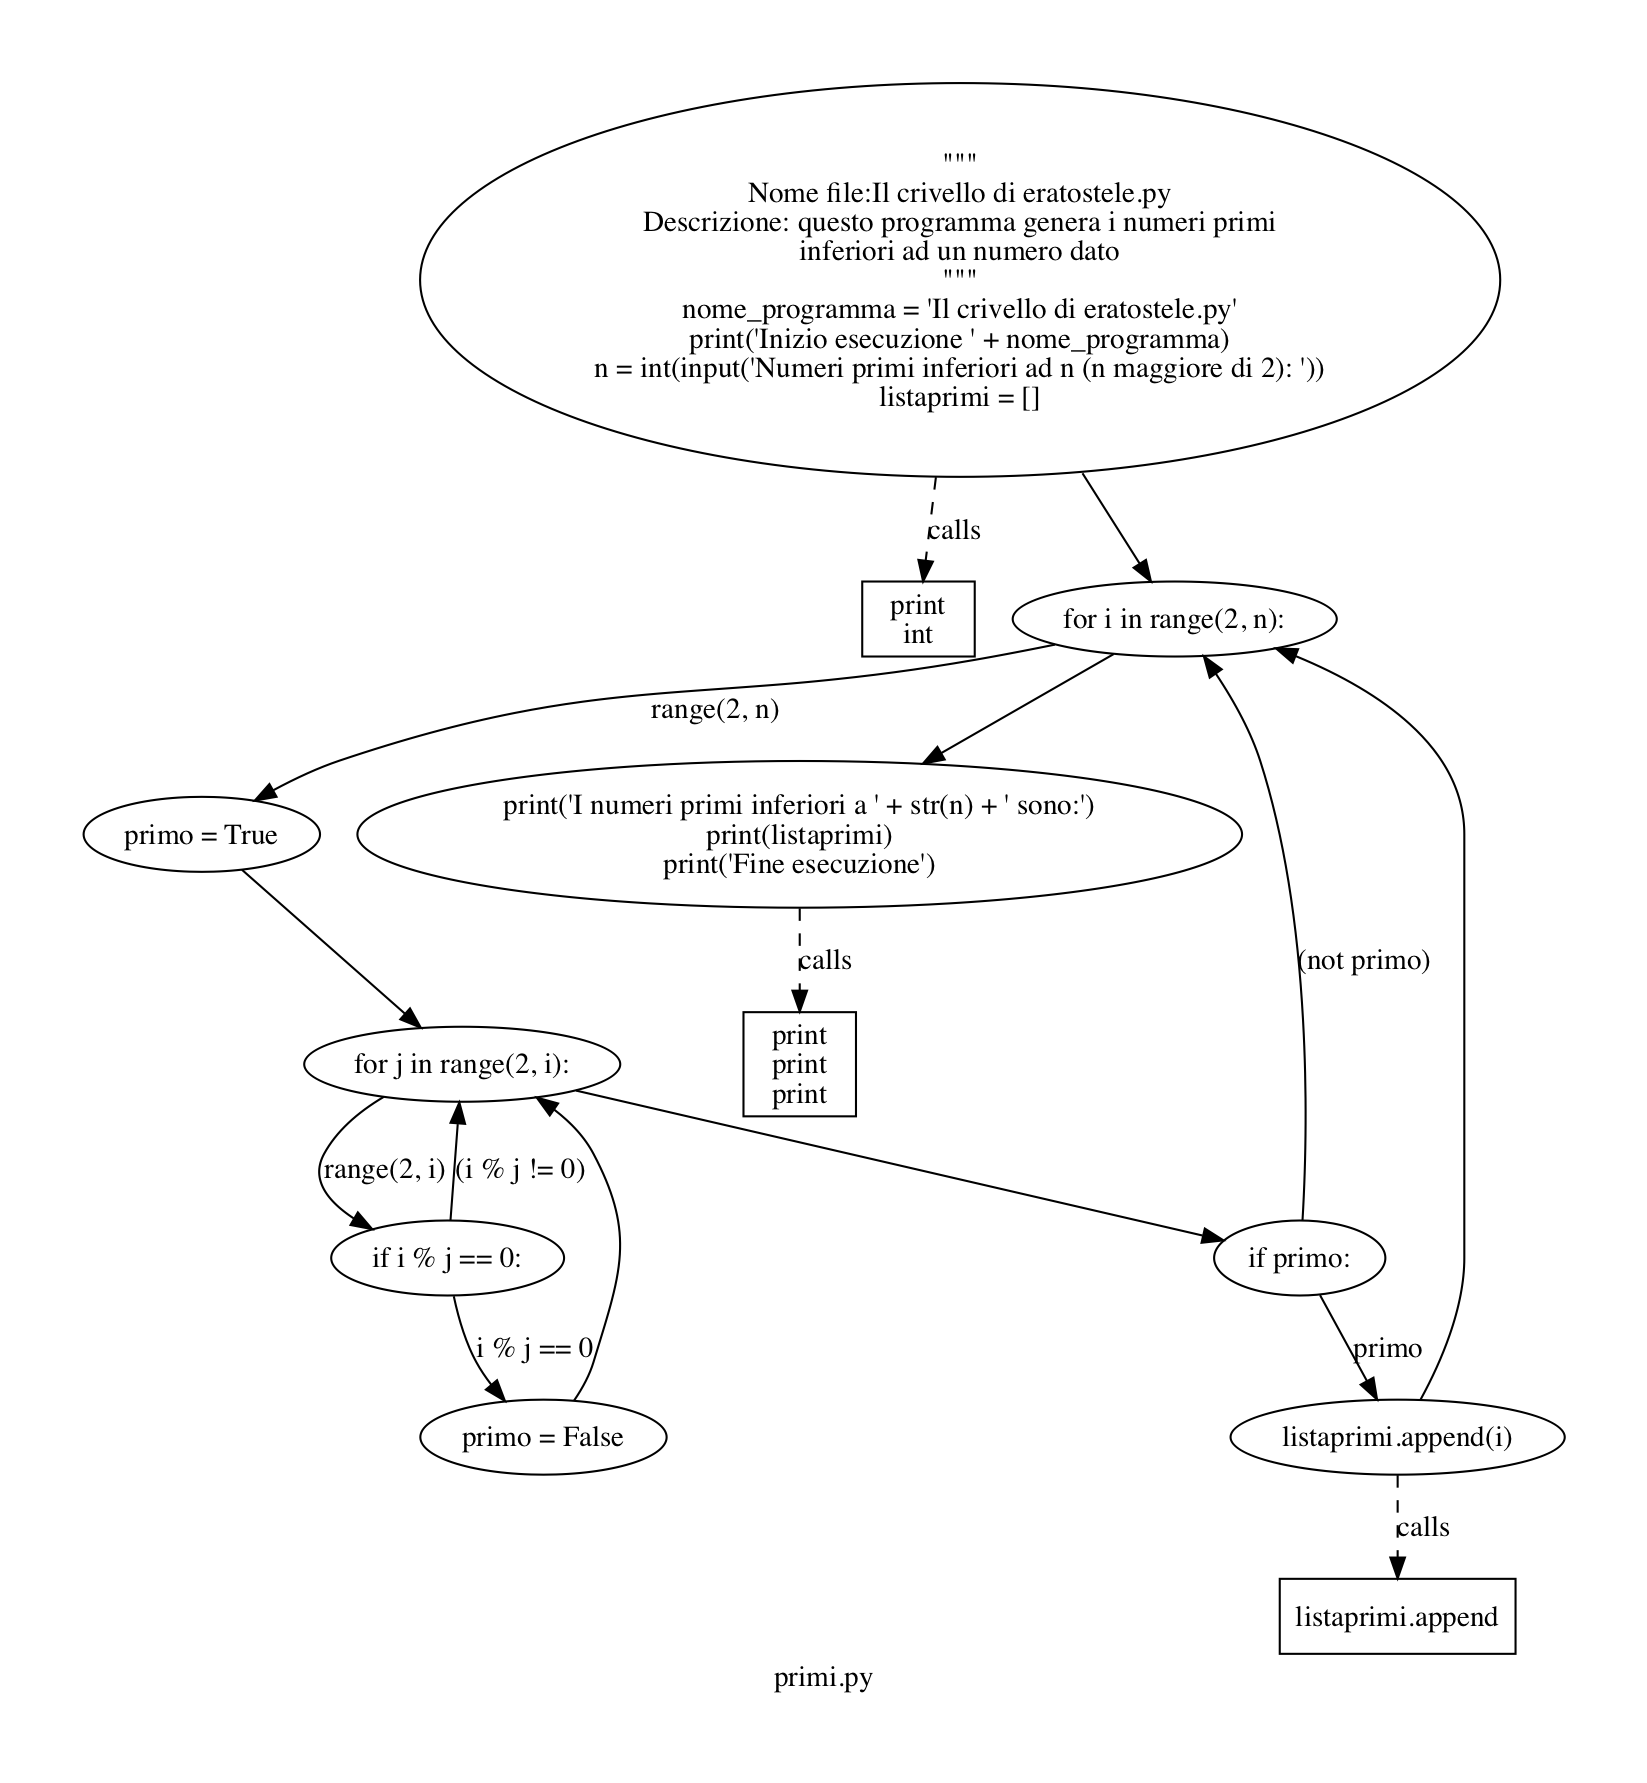
\includegraphics[height=18cm, width=9cm, keepaspectratio]{img/primi.png}
\end{figure}

Lanciamo il nostro offuscatore:

\begin{graybox}
\begin{lstlisting}[language=bash,basicstyle=\fontsize{10}{9}\selectfont,]
python3  		offuscatore.py 	primi.py
\end{lstlisting}
\end{graybox}

E otteniamo questo risultato:

\begin{graybox}
\begin{lstlisting}[language=bash,basicstyle=\fontsize{10}{9}\selectfont,]
from random import randint
from random import SystemRandom
O00OOO000O0000OO0OOOOO0 = 10
OO0O00O000O00OOOOO0O00O = [36, 58, 1, 46, 23, 5, 16, 65, 2, 41, 2, 7, 1, 37,
    0, 11, 16, 2, 21, 16]
OO00O000O00000O00O0O000 = 'Il crivello di eratostele.py'
print('Inizio esecuzione ' + OO00O000O00000O00O0O000)
if OO0O00O000O00OOOOO0O00O[3] % OO0O00O000O00OOOOO0O00O[5
    ] == OO0O00O000O00OOOOO0O00O[2]:
    OO0O00O000O00OOOOO0O00O[5] = OO0O00O000O00OOOOO0O00O[1
        ] * OO0O00O000O00OOOOO0O00O[4] % OO0O00O000O00OOOOO0O00O[11
        ] + OO0O00O000O00OOOOO0O00O[6] % OO0O00O000O00OOOOO0O00O[5]
    OO0O00O000O00OOOOO0O00O[14] = randint(0, 100)
    OO0O00O000O00OOOOO0O00O[4] = randint(0, 10) * OO0O00O000O00OOOOO0O00O[11
        ] + OO0O00O000O00OOOOO0O00O[8]
    OO0O0O0O00O0OO00OO0O00O = (OO0O00O000O00OOOOO0O00O[4] +
        OO0O00O000O00OOOOO0O00O[7] + OO0O00O000O00OOOOO0O00O[10]
        ) % OO0O00O000O00OOOOO0O00O[11]
    O0OOOOOOO0OO0O00O000OO0 = (OO0O0O0O00O0OO00OO0O00O + 
        OO0O00O000O00OOOOO0O00O[3] % OO0O00O000O00OOOOO0O00O[5])
    OO0OO0O00000O0O00O00O0O = OO0O0O0O00O0OO00OO0O00O * O0OOOOOOO0OO0O00O000OO0
O00000O0O0000O0000O00O0 = int(input(
    'Numeri primi inferiori ad n (n maggiore di 2): '))
if OO0O00O000O00OOOOO0O00O[3] % OO0O00O000O00OOOOO0O00O[5
    ] == OO0O00O000O00OOOOO0O00O[2]:
    OO0O00O000O00OOOOO0O00O[5] = OO0O00O000O00OOOOO0O00O[1
        ] * OO0O00O000O00OOOOO0O00O[4] % OO0O00O000O00OOOOO0O00O[11
        ] + OO0O00O000O00OOOOO0O00O[6] % OO0O00O000O00OOOOO0O00O[5]
    OO0O00O000O00OOOOO0O00O[14] = randint(0, 100)
    OO0O00O000O00OOOOO0O00O[4] = randint(0, 10) * OO0O00O000O00OOOOO0O00O[11
        ] + OO0O00O000O00OOOOO0O00O[8]
    OO0O0O0O00O0OO00OO0O00O = (OO0O00O000O00OOOOO0O00O[4] +
        OO0O00O000O00OOOOO0O00O[7] + OO0O00O000O00OOOOO0O00O[10]
        ) % OO0O00O000O00OOOOO0O00O[11]
    O0OOOOOOO0OO0O00O000OO0 = (OO0O0O0O00O0OO00OO0O00O + 
        OO0O00O000O00OOOOO0O00O[3] % OO0O00O000O00OOOOO0O00O[5])
    OO0OO0O00000O0O00O00O0O = OO0O0O0O00O0OO00OO0O00O * O0OOOOOOO0OO0O00O000OO0
OOO000O0O0OO0O0OO00O000 = []
for i in range(2, O00000O0O0000O0000O00O0):
    O0OO0OOOOOOOO00OOOO0OOO = True
    for j in range(2, i):
        if i % j == 0:
            O0OO0OOOOOOOO00OOOO0OOO = False
    if O0OO0OOOOOOOO00OOOO0OOO:
        OOO000O0O0OO0O0OO00O000.append(i)
print('I numeri primi inferiori a ' + str(O00000O0O0000O0000O00O0) + ' sono:')
print(OOO000O0O0OO0O0OO00O000)
print('Fine esecuzione')
\end{lstlisting}
\end{graybox}

Se eseguiamo i due codici la semantica viene mantenuta. La struttura del control flow graph esplode.

\begin{figure}[!h]
        \centering
        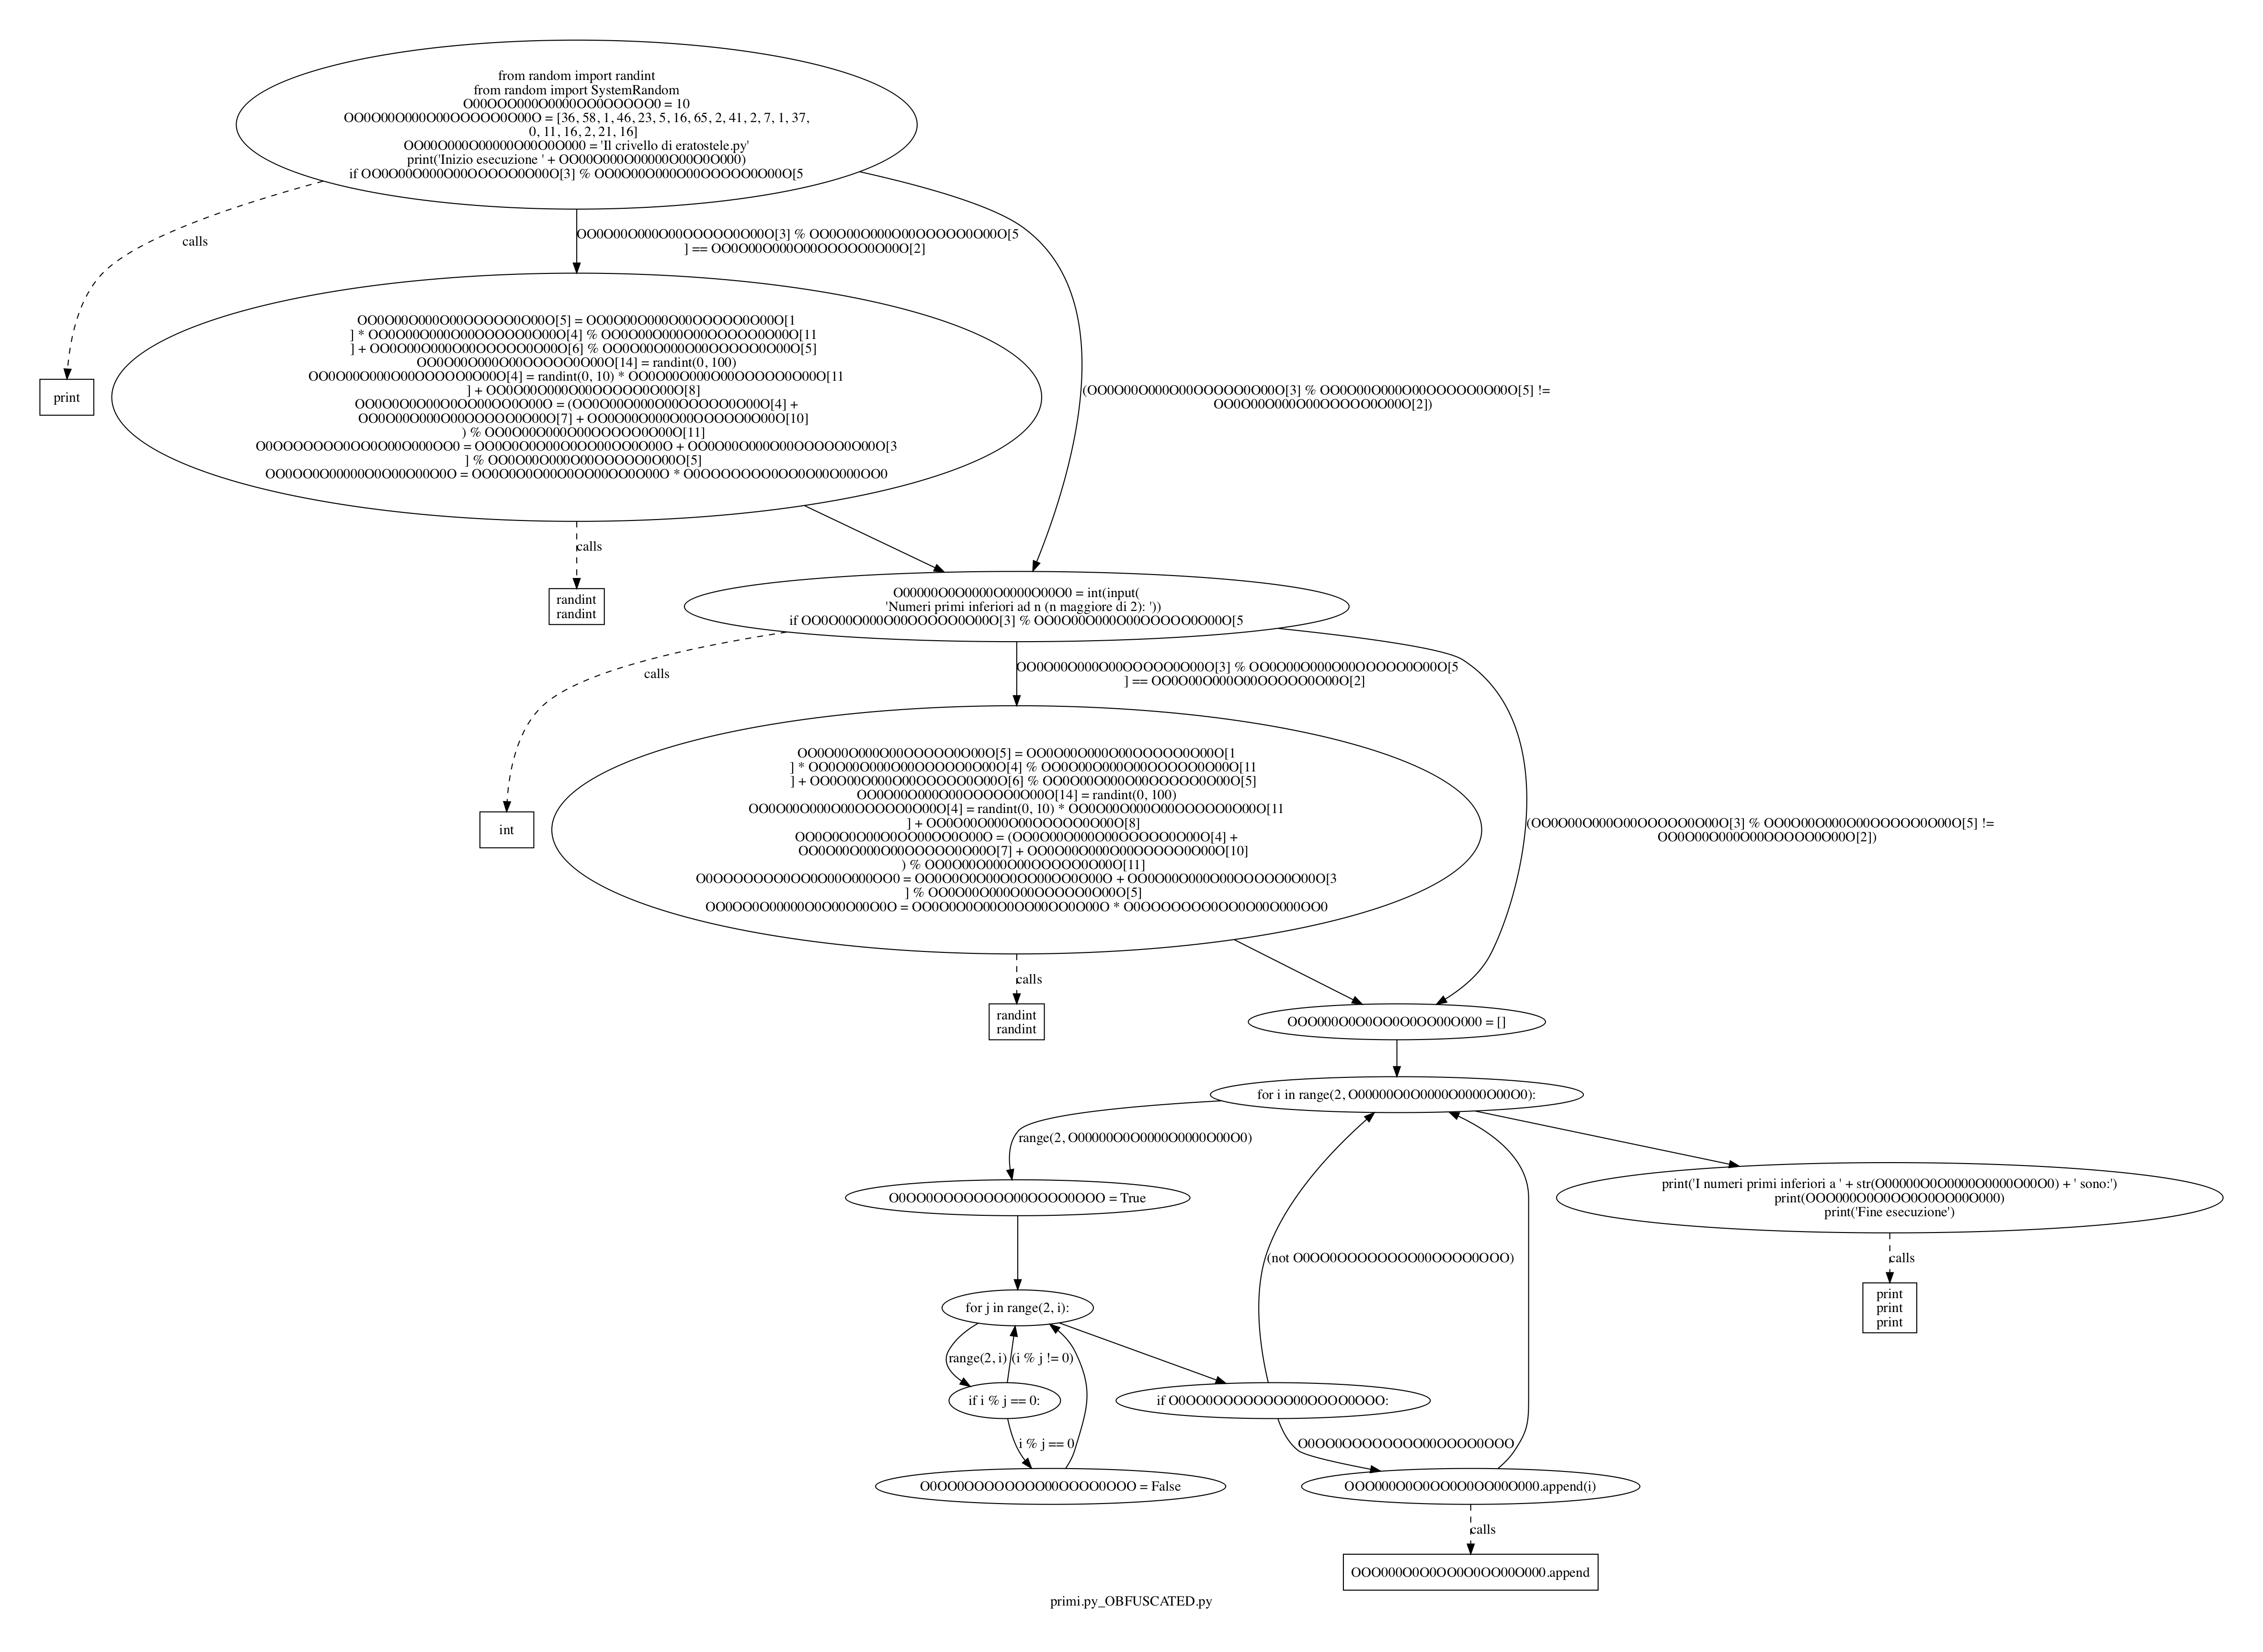
\includegraphics[height=24cm, width=15cm, keepaspectratio]{img/primi_OBFUSCATED.png}
\end{figure}


% BIBLIOGRAFIA
%\addcontentsline{toc}{chapter}{\bibname}
%\begin{thebibliography}{9}

%\end{thebibliography}


\end{document}